\subsection{Discrete adjoint solutions on a shock cube problem}
\label{subsection:Discrete_Adjoint}

Following the adjoint formulation explained in Section \ref{section:Adjoint} it is seen that the adjoint formulation (also known as the \textit{dual problem}) can be written as a linear system:

\begin{equation}
\mathbf{A}^T\mathbf{x} = -\mathbf{b}^T
\end{equation}

Thus we can write the transpose of the residual Jacobian matrix, ${\partial{R}}/{\partial{U}}$ as matrix $A^T$ and the right hand side vector $\mathbf{b}$ as the derivative of the functional with respect to the state, ${\partial{J}}/{\partial{\mathbf{U_i}}}$\par

Adjoint sensitivities were evaluated for a shock cube problem governed by the Euler equations (see figure \ref{fig:Adjoints}). The initial conditions were ${\rho_R}/{\rho_L} = 8$, ${P_R}/{P_L} = 10$. Average pressure in the entire domain was selected as the functional, $J$. \par

\begin{figure}[t!]
  \centering
   \subfigure[Initial conditions for density showing large jump between left and right states]
   {\label{fig:init_cond}	   
   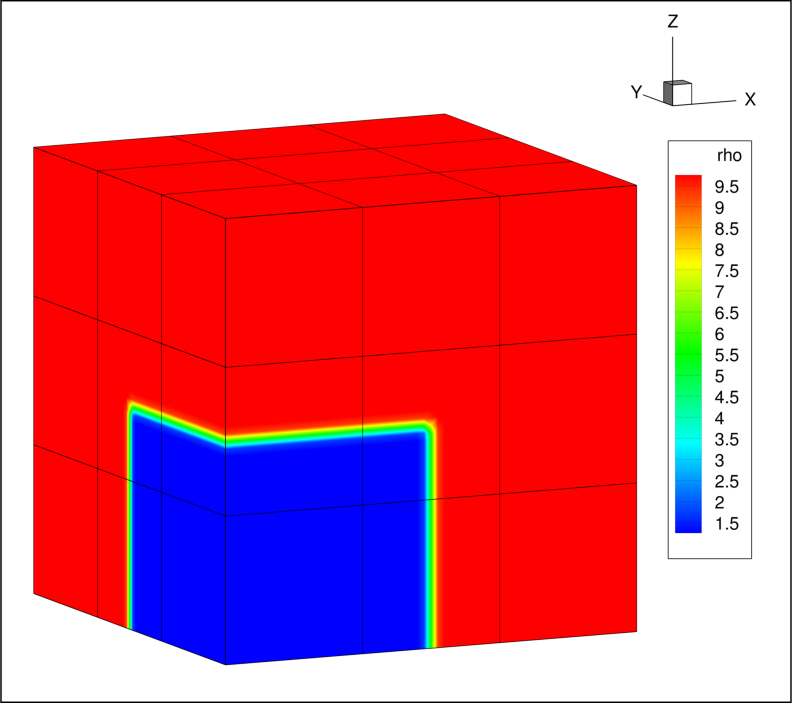
\includegraphics[height=0.45\textwidth]{figs/20Rho.png}}%
   \subfigure[sensitivity to Density]
   {\label{fig:rho_Adjoint}	   
   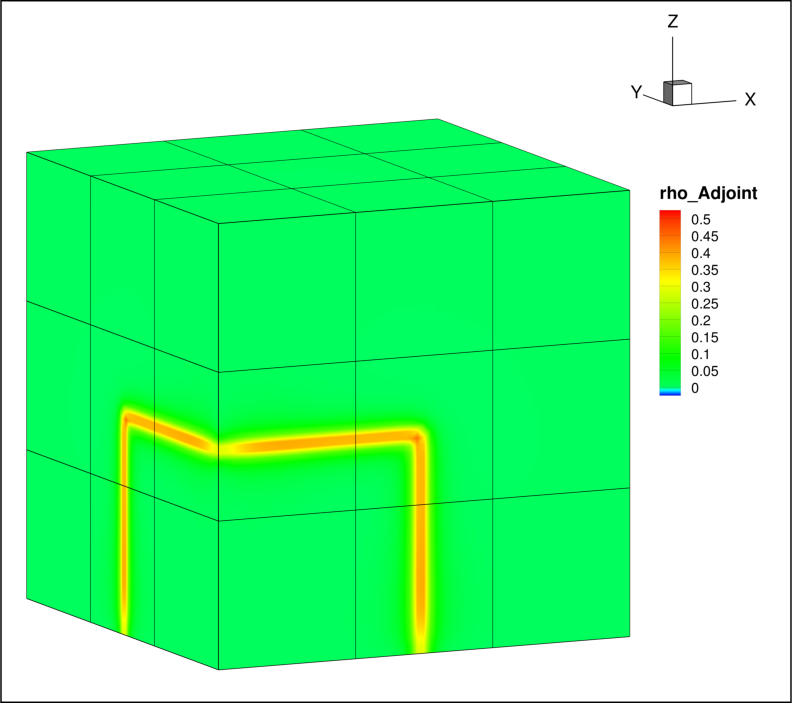
\includegraphics[height=0.45\textwidth]{./figs/20RhoAdj.png}}%
\caption{Contours of $\rho$ and adjoint $\psi_{\rho}$ at t = 0 sec. 27 (20x20x20) blocks} 
\label{fig:Adjoints}      
\end{figure}  